\documentclass[aps,preprint,nofootinbib,floatfix]{revtex4-1}

%\usepackage{cite}
\usepackage[pdftex]{graphicx}
\graphicspath{{./figures/}}
%\graphicspath{{./}}
\usepackage{amsmath,amssymb,amsfonts,amsthm,amscd,bm}
\usepackage{algorithm}
\usepackage{algorithmic}
%\usepackage{epstopdf}
%\usepackage{fixltx2e}
%\usepackage{stfloats}

\hyphenation{op-tical net-works semi-conduc-tor}

\newtheorem{theorem}{Theorem}
\newtheorem{definition}[theorem]{Definition}
\newtheorem{assumption}[theorem]{Assumption}
\newtheorem{lemma}[theorem]{Lemma}
\newtheorem{corollary}[theorem]{Corollary}
\newtheorem{proposition}[theorem]{Proposition}
\newtheorem{conjecture}[theorem]{Conjecture}
\newtheorem{remark}[theorem]{Remark}
\newtheorem{example}{Example}

%% our definitions %%%%%%%%%%%%%%%%%%%%%%%%%%%%%%%%%%%%%%%%%%%%%%%%%%%%%%%%%%%%
\DeclareMathOperator{\aff}{aff}
\DeclareMathOperator{\st}{s.t.}
\DeclareMathOperator{\LC}{LC}
\DeclareMathOperator{\affnot}{aff_0}
\DeclareMathOperator{\conv}{conv}
\DeclareMathOperator{\relint}{relint}
\DeclareMathOperator{\vol}{vol}
\DeclareMathOperator{\range}{range}
\DeclareMathOperator{\image}{im}
\DeclareMathOperator{\nullspace}{null}
\DeclareMathOperator{\area}{area}
\DeclareMathOperator{\vspan}{span}
\DeclareMathOperator{\id}{Id}
\DeclareMathOperator{\cond}{cond}
\DeclareMathOperator{\prox}{prox}
\DeclareMathOperator*{\argmax}{arg\,max}
\DeclareMathOperator*{\argmin}{arg\,min}
\DeclareMathOperator*{\minimize}{minimize}
\DeclareMathOperator{\diag}{diag}
\DeclareMathOperator{\Tr}{Tr}

\graphicspath{{figs/}}

\begin{document}

\title{One Dimensional Random Projection and Clustering}

%\author{}
%\email{guifranca@gmail.com}
%\affiliation{Johns Hopkins University, Center for Imaging Science}

\begin{figure}
\begin{minipage}{.49\textwidth}
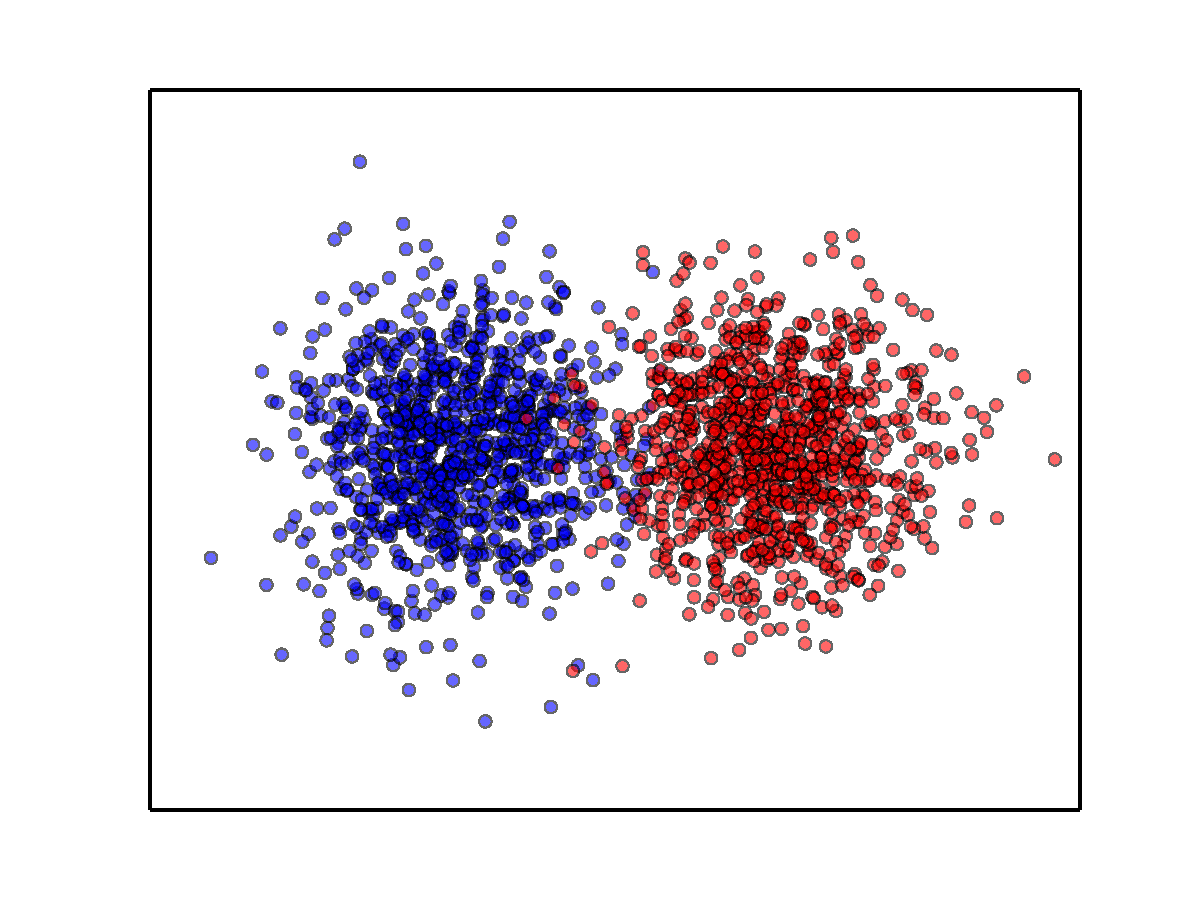
\includegraphics[scale=.45]{2d_gauss_separate.pdf}
\end{minipage}
\begin{minipage}{.49\textwidth}
\begin{tabular}{ c | c | c | c }
~$n$~ & $k$-means & PCA $k$-means & RAN $k$-means \\
\hline
1 & 0.9735 & 0.9735 & 0.9745 \\
2 & 0.982 & 0.9815 & 0.9825 \\
3 & 0.9785 & 0.9785 & 0.982 \\
\hline
\end{tabular}
\end{minipage}
\caption{\label{fig:2d_gauss_sep}
We have $x \sim \tfrac{1}{2}\left( \mathcal{N}(\mu_1, I) +
\mathcal{N}(\mu_2, I)\right)$ where $\mu_1 = (0,0)^T$ and $\mu_2=(4,0)^T$,
and $1000$ points on each cluster.
}
\end{figure}

\begin{figure}
\begin{minipage}{.49\textwidth}
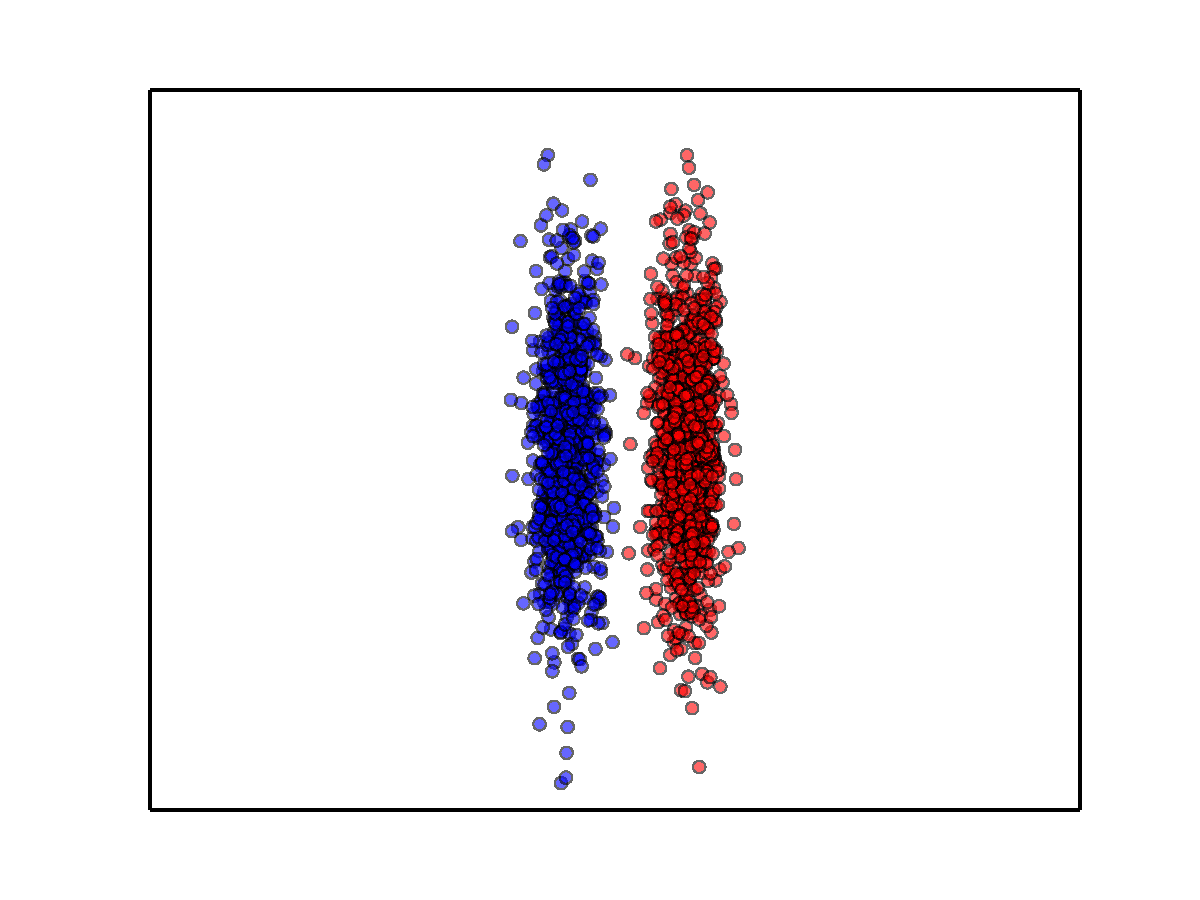
\includegraphics[scale=.45]{2d_cigar.pdf}
\end{minipage}
\begin{minipage}{.49\textwidth}
\begin{tabular}{ c | c | c | c }
~$n$~ & $k$-means & PCA $k$-means & RAN $k$-means \\
\hline
1 & 0.5265 & 0.5215 & 1.0 \\
2 & 0.5285 & 0.5285 & 1.0 \\
3 & 0.5285 & 0.513 & 1.0 \\
\hline
\end{tabular}
\end{minipage}
\caption{\label{fig:2d_gauss_sep}
We have $x \sim \tfrac{1}{2}\left( \mathcal{N}(\mu_1, \Sigma) +
\mathcal{N}(\mu_2, \Sigma)\right)$ where $\mu_1 = (0,0)^T$, $\mu_2=(5,0)^T$,
and $\Sigma = \left( \begin{smallmatrix} 1/2 & 0 \\ 0 & 15 \end{smallmatrix}
\right)$,
and $1000$ points on each cluster.
}
\end{figure}

\begin{figure}
\begin{minipage}{.49\textwidth}
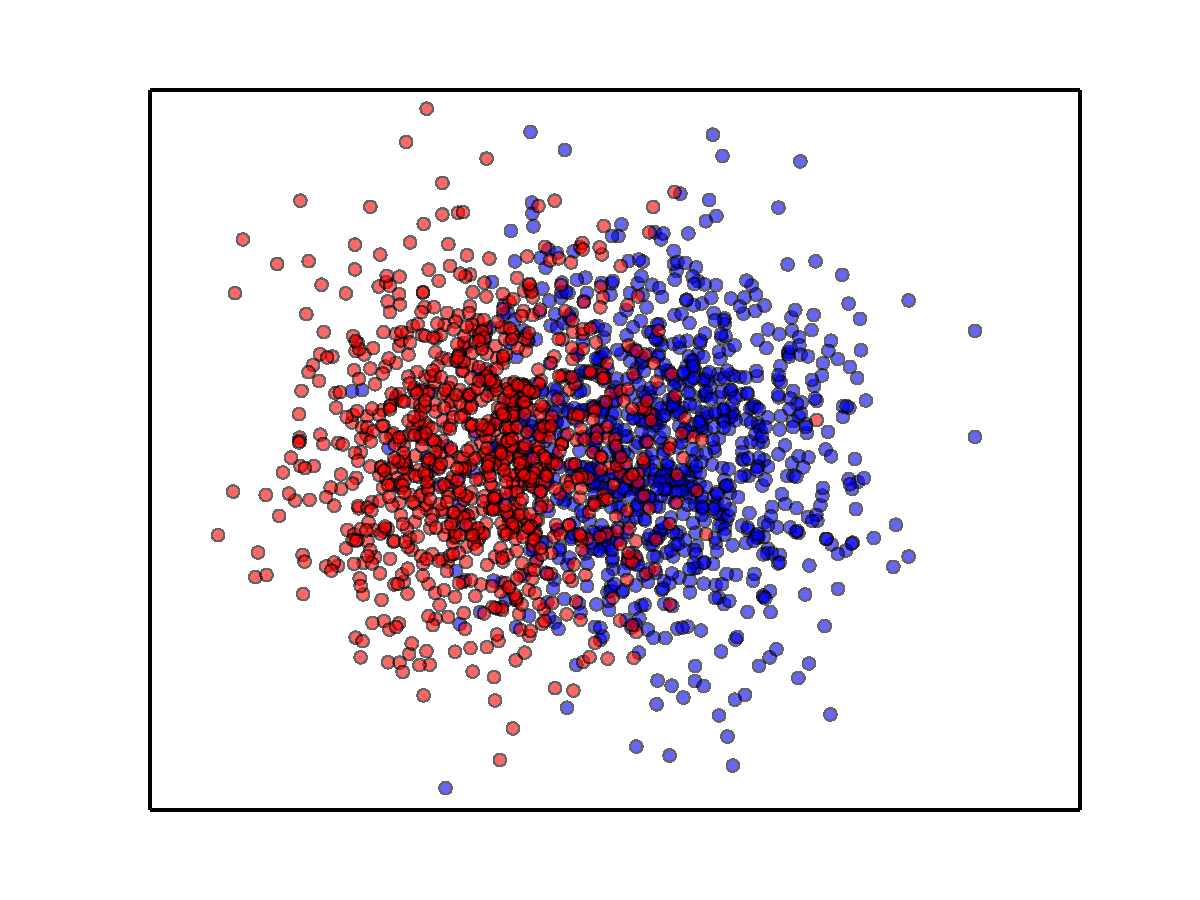
\includegraphics[scale=.45]{30d_gauss.pdf}
\end{minipage}
\begin{minipage}{.49\textwidth}
\renewcommand*{\arraystretch}{.3}
\begin{tabular}{ c | c | c | c }
~$D$~ & $k$-means & PCA $k$-means & RAN $k$-means \\
\hline
5 & 0.84 & 0.8415 & 0.841 \\
10 & 0.844 & 0.846 & 0.7985 \\
15 & 0.8325 & 0.8365 & 0.7465 \\
20 & 0.846 & 0.85 & 0.764 \\
25 & 0.8555 & 0.8505 & 0.714 \\
30 & 0.825 & 0.8225 & 0.728 \\
50 & 0.8485 & 0.8465 & 0.6775 \\
100 & 0.832 & 0.8325 & 0.644 \\
200 & 0.8085 & 0.8145 & 0.592 \\
300 & 0.7645 & 0.794 & 0.5755 \\
500 & 0.6915 & 0.756 & 0.5615 \\
1000 & 0.5075 & 0.6965 & 0.562 \\
2000 & 0.5495 & 0.662 & 0.543 \\
5000 & 0.531 & 0.5135 & 0.539 \\
\hline
\end{tabular}
\end{minipage}
\caption{\label{fig:2d_gauss_sep}
High dimensions.
We have $x \sim \tfrac{1}{2}\left( \mathcal{N}(\mu_1, I_D) +
\mathcal{N}(\mu_2, I_D)\right)$ where $\mu_1 = (0,0,\dotsc,0)^T$,
$\mu_2=(1,0,\dots,0)^T$,
and $1000$ points on each cluster. We show only the two principal components
of the data in the plot above.
}
\end{figure}

\end{document}
